\section{Discusión}
\subsubsection{Discusión de la generación y etiquetado del conjunto de datos.}
\label{sec:discusion}
La detección de áreas quemadas en cultivos de caña de azúcar presenta un desafío significativo, principalmente debido a la necesidad de 
disponer de una base de datos confiable y de alta calidad. En este estudio, se propuso una metodología específica para la selección de 
imágenes con el objetivo de etiquetar correctamente las áreas quemadas. 

A pesar de los esfuerzos por utilizar grandes conjuntos de datos globales de áreas quemadas, como los presentados en el trabajo de \citet{arnaudo_robust_2023}, 
la aplicación de estos datos a los modelos individuales enfrenta limitaciones significativas. Los estudios globales a menudo se centran en grandes incendios forestales 
que cubren extensiones superiores a las 5,000 hectáreas \citet{seydi_burnt-net_2022}. Este enfoque no es el ideal para el contexto de 
la detección de quema en cultivos de caña de azúcar, donde las áreas quemadas son generalmente mucho más pequeñas, menores a 100 hectáreas y con condiciones locales propias. 
Como resultado, las etiquetas utilizadas en estudios globales no logran capturar con precisión los detalles de áreas quemadas de menor escala (ver Figura \ref{fig:db}), lo cual es crítico en este 
contexto.

\begin{figure}[H]
    \centering    
    \caption{Ejemplo de etiquetado de áreas quemadas a nivel mundial.}
    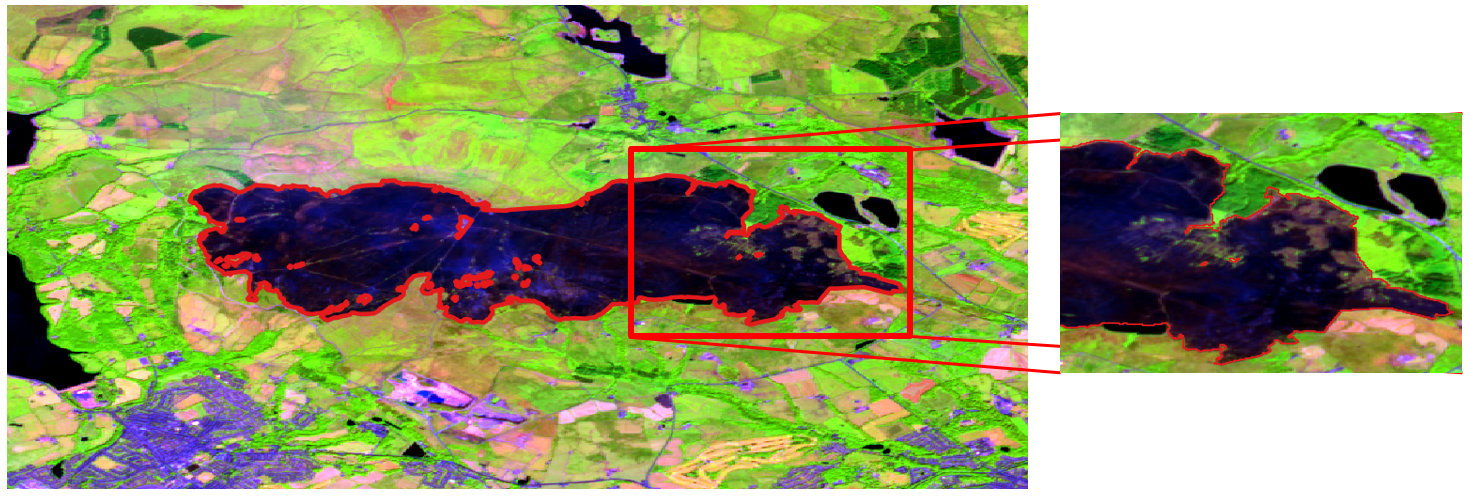
\includegraphics[width=1\textwidth]{img/8_capitulo6/basedatos.png}
    \label{fig:db}
    \begin{flushleft}
        \vspace{-\baselineskip}
        \textit{Nota.} Se visualiza la etiqueta EMSR291\_AOI02\_01 de $714$ ha de área quemada. Extraído de \citet{arnaudo_robust_2023}.      
        \vspace{-\baselineskip}
    \end{flushleft}        
\end{figure}

El etiquetado de nuestra base de datos se realizó mediante el uso de “scribbles”, lo cual en áreas no etiquetadas puede llevar a definiciones poco claras sobre qué debe 
considerarse como quema. Este problema es general en la segmentación de áreas quemadas como se discute en \citet{knopp_deep_2020}, 
donde la ambigüedad no solo se limita a las áreas parcialmente afectadas por el fuego, sino que también se extiende a las áreas quemadas con cierta antigüedad, donde es crucial 
definir en qué momento una zona previamente quemada se ha recuperado lo suficiente para dejar de ser clasificada como área quemada.

En el contexto nacional, la caña de azúcar no tiene un período de zafra único, lo que significa que la quema de caña y su cosecha pueden ocurrir en cualquier época del año \citep{helfgott_cultivo_2016};
esto complica aún más la interpretación de las áreas quemadas, especialmente en la diferenciación con suelos desnudos que se están recuperando y reacondicionando para la siembra de nueva caña soca que no es
visible hasta el primer mes en las etapas de macollamiento y crecimiento. 

Durante el período de cosecha, las quemas y requemas son comunes, lo que implica que el suelo desnudo con residuos de caña (straw) suele preceder a la quema, al igual que ocurre con la caña madura como se ha visto
en los resultados de la Sección \ref{sec:area_validacion}. Por lo tanto, que la imagen anterior a la quema no muestre vegetación no excluye la posibilidad de que se trate de un área quemada (ver Figura \ref{fig:caña}). 

\begin{figure}[H]
    \centering    
    \caption{Ejemplo de distintos estados del área de cultivo de caña de azúcar durante la época de cosecha.}
    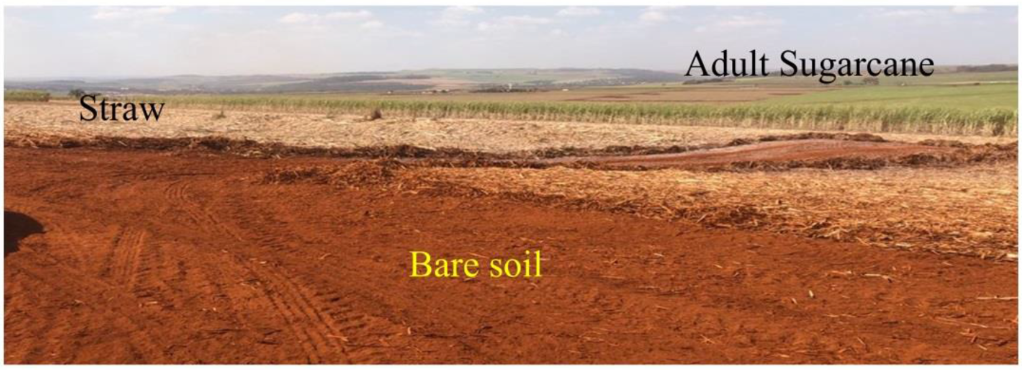
\includegraphics[width=1\textwidth]{img/8_capitulo6/posibilidades.png}
    \label{fig:caña}
    \begin{flushleft}
        \vspace{-\baselineskip}
        \textit{Nota.} La imagen muestra tres estados: caña de azúcar madura (adult sugarcane), suelo desnudo (bare soil) y residuos de caña (straw). Extraído de \citet{campos_detection_2022}.
        \vspace{-\baselineskip}
    \end{flushleft}
\end{figure}

\subsubsection{Discusión de los resultados de los modelos base.}
En cuanto a los resultados del modelo U-Net, se observa que produce una segmentación de áreas quemadas más gruesa en comparación con una clasificación basada en píxeles, lo cual coincide con los hallazgos de 
\citet{knopp_deep_2020}. Esto se evidencia aún más con el modelo LightGBM delimitando de manera fina las áreas de cultivo extensas diferenciándolos de los píxeles que pertenecen a los caminos que cruzan los campos de cultivo.

Este estudio representa un primer intento en el campo de la teledetección de combinar LightGBM y U-Net mediante un enfoque de stacking. Según \citet{zhang_review_2022}, el stacking 
permite combinar las fortalezas de diferentes modelos base, mejorando significativamente la precisión de las predicciones en comparación con el uso de modelos individuales. 

Al utilizar U-Net, que captura bien las relaciones no lineales en las imágenes, junto con LightGBM, un potente algoritmo de aprendizaje automático para la clasificación por píxel, se pueden aprovechar las capacidades complementarias de ambos modelos, logrando 
un equilibrio más robusto y flexible en la detección de áreas quemadas en cultivos de caña de azúcar. 

Sin embargo, el fenómeno de ``salt n' pepper'', como señala \citet{sdraka_floga_2024}, es un inconveniente significativo que introduce ruido en la clasificación de píxeles y dificulta una delimitación precisa de las áreas quemadas. Este error se propaga a partir 
de los índices espectrales y afecta especialmente a los modelos de aprendizaje automático, como LightGBM y la regresión logística, provocando confusión entre áreas quemadas y superficies similares, como cuerpos de agua, sombras y estructuras urbanas. 

Aunque el modelo ensamblado de stacking, que combina U-Net como algoritmo de deep learning, puede mitigar este problema en cierta medida, sigue siendo susceptible a este tipo de ruido, especialmente en situaciones con alta confusión espectral o condiciones de imagen 
complejas.

Las variables del modelo LightGBM se alinean con la literatura existente sobre la detección de áreas quemadas, en la que la mayoría de los estudios se enfocan en utilizar bandas visibles, así como bandas en el rango del infrarrojo cercano, borde rojo, y de onda corta
debido a su mayor sensibilidad para detectar quemas, como se ha demostrado en investigaciones previas \citep{van_dijk_spectral_2021,QUINTANO20111597}. Además, es habitual incluir índices como el NDVI y el NBR para mejorar la precisión en la identificación de áreas quemadas \citep{lee_machine_2022}. 

La mayor relevancia de la distancia a las coberturas agrícolas en el modelo se debe a su enfoque en priorizar las quemas dentro de las áreas de cultivos y diferenciar los terrenos eriazos con suelos desnudos ajenos a las áreas de cultivo.


\subsubsection{Discusión de los resultados del modelo Stacking y su validación.}

El modelo ensamblado de Stacking supera cuantitativamente a cada uno de estos modelos individuales (Tabla \ref{tab:evaluacion_modelos}). En particular, posee un \textbf{F1-Score} de $90.6\%$, lo cual es adecuado para garantizar valores consistentes y reducir el impacto de falsas alarmas al combinar múltiples 
modelos de detección. Como se menciona en estudios anteriores, el uso de técnicas de ensemble learning puede mejorar significativamente la precisión y robustez en la detección de áreas quemadas \citep{lee_machine_2022}

Mediante los reportes del OEFA, se validó que el modelo muestra un buen rendimiento con la mayoría de los umbrales. Un mayor umbral ayuda a eliminar falsos positivos, lo cual es útil en áreas donde la cobertura es similar, como suelo desnudo o sombras de nubes, 
y se requiere discriminar la quema de manera consistente, como en el caso de la emergencia \textbf{0546}. 

Por otro lado, umbrales más bajos son más efectivos para delimitar correctamente áreas quemadas en zonas con mezcla de vegetación, 
como se observa con el umbral de la emergencia \textbf{0068}.

En la Figura \ref{fig:umbral}, se evidencia que el modelo ensamblado está alineado con la información proporcionada por la OEFA y supera a los modelos utilizados basados en reglas más comunes, como el BADI, mostrando su eficacia en escenarios complejos y su capacidad 
para integrar diferentes fuentes de información para una mejor detección y delimitación de áreas quemadas.

\begin{figure}[H]
    \centering
    \caption{Ejemplo de la detección de áreas quemadas en la costa norte y centro del Perú.}
    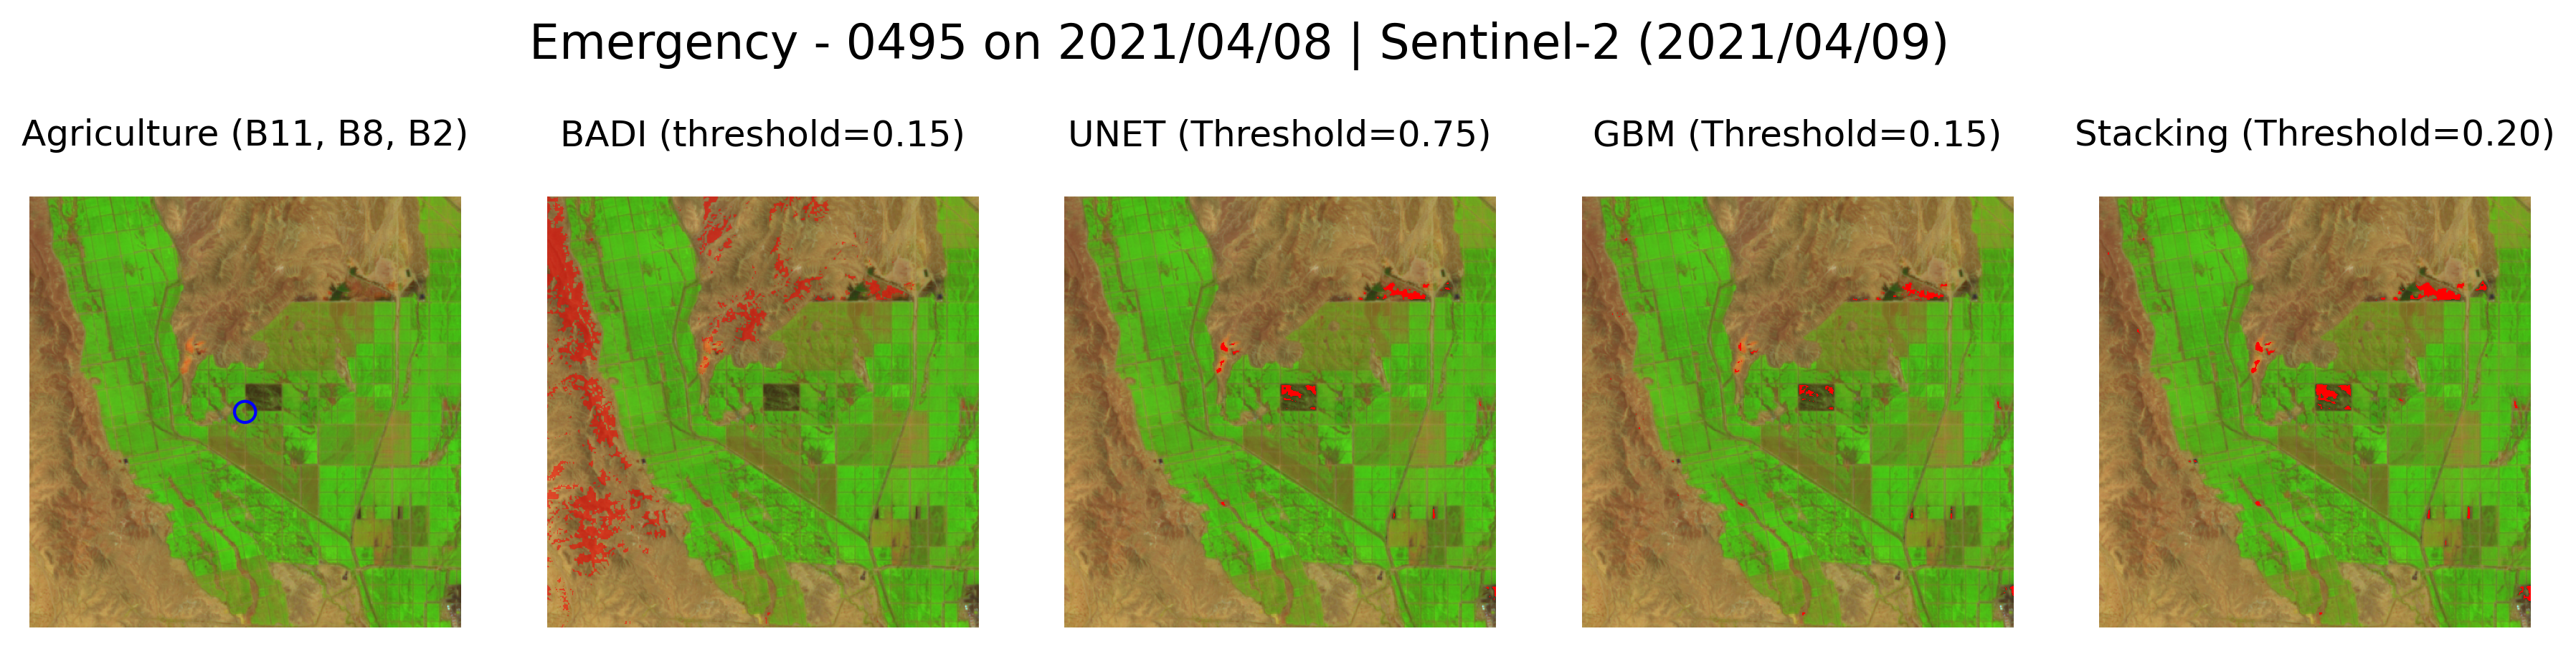
\includegraphics[width=1.01\textwidth]{img/8_capitulo6/0495.png}
    \label{fig:umbral}
    \begin{flushleft}
        \vspace{-\baselineskip}
        \textit{Nota.} Se visualiza la detección de áreas quemadas en tres áreas de validación con diferentes umbrales de probabilidad. Elaboración propia.
        \vspace{-\baselineskip}
    \end{flushleft}
\end{figure}

\subsubsection{Discusión de la inferencia en el área piloto.}
Inicialmente, al aplicar un filtro de nubosidad inferior al 10\% para seleccionar imágenes satelitales de Sentinel-2 en el período de enero de 2023 a agosto de 2024, se lograron obtener solo 
96 imágenes de las 222 disponibles, que se redujeron a 30 de acuerdo a los criterios de la Sección \ref{sec:inferencia}. Esta limitación se debe a la alta presencia de nubosidad en la región de estudio, 
lo que complica la obtención de imágenes satelitales claras y de alta calidad. A pesar de estas restricciones, el modelo ensamblado fue capaz de detectar áreas quemadas en la región piloto 
utilizando las imágenes seleccionadas.

En la inferencia del área piloto, se observó que el modelo ensamblado es especialmente eficaz para detectar la ubicación de eventos de quema, resultando útil para identificar y 
delimitar tanto quemas activas como recientes, principalmente en áreas mayores a 1 ha. El modelo se distingue claramente al diferenciar áreas quemadas de otras superficies, como zonas urbanas,
cuerpos de agua y suelo desnudo fuera de las áreas de cultivo, lo que proporciona una alta fiabilidad en la toma de decisiones en estos escenarios.

El uso de umbrales altos de probabilidad en la inferencia permitió minimizar los falsos positivos y mejorar la precisión en la detección de áreas quemadas, lo cual es crucial para la toma de decisiones. Sin embargo, 
dependiendo de la situación, se puede ajustar el umbral para priorizar una detección más amplia o una más precisa. Esta elección depende de si se prefiere obtener más puntos de datos para un análisis exhaustivo o si 
se requiere mayor exactitud en la identificación de áreas quemadas. 

La decisión final debe alinearse con las necesidades de fiscalización y monitoreo de las empresas azucareras administradas por el OEFA.
